% pdflatex abra.tex
% convert -density 300x300 -alpha off abra.pdf abra.png
\documentclass[border={2pt 2pt 2pt 2pt}]{standalone}
\usepackage{tikz}
\usetikzlibrary{calc}
\begin{document}

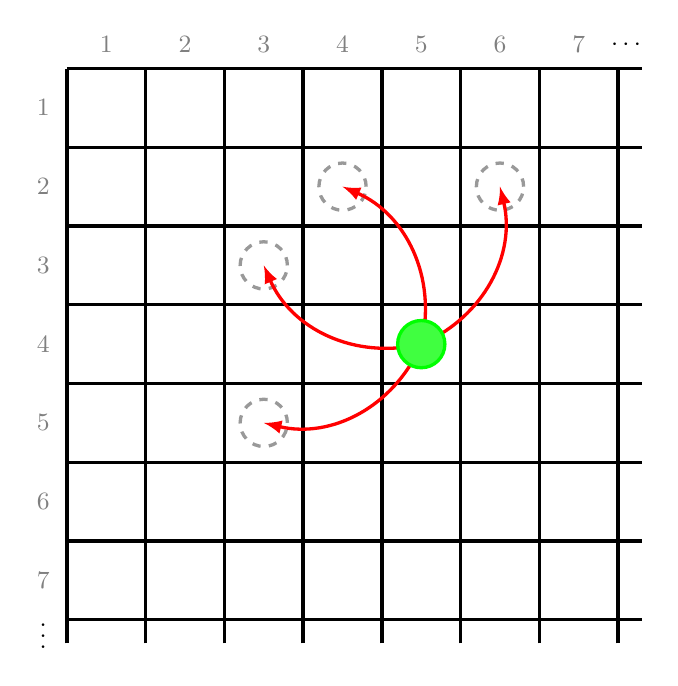
\begin{tikzpicture}[very thick]
\draw (0,-0.3) grid (7.3,7);
\draw[black!40,dashed] (2.5,4.5) circle [radius=.3];
\draw[black!40,dashed] (2.5,2.5) circle [radius=.3];
\draw[black!40,dashed] (3.5,5.5) circle [radius=.3];
\draw[black!40,dashed] (5.5,5.5) circle [radius=.3];
\draw[red,-latex] (4.5,3.5) to [bend left=40] (2.5,4.5);
\draw[red,-latex] (4.5,3.5) to [bend left=40] (2.5,2.5);
\draw[red,-latex] (4.5,3.5) to [bend right=40] (3.5,5.5);
\draw[red,-latex] (4.5,3.5) to [bend right=40] (5.5,5.5);
\draw[green,very thick,fill=green!75] (4.5,3.5) circle [radius=.3];
%\node at (0.5,6.5) {\small(1,1)};
\foreach \x in {1,...,7} {
  \node[gray] at (\x-0.5,7.3) {\small\x};
  \node[gray] at (-0.3,7.5-\x) {\small\x};
}
\node at (7.1,7.3) {\small$\cdots$};
\node at (-0.3,-0.1) {\small$\vdots$};
\end{tikzpicture}

\end{document}
